\section{Gamification}
\label{sec:gamification}
Gamification is "the process of game-thinking and game mechanics to engage users and solve problems" \cite{Zichermann2011}, i.e. using core elements of games to attract users and keep them coming back to a specific task. Since making our final product engaging is one of our requirements, gamefication is a natural way of approaching the problem of making something educational engaging.\newline

Gamification is used in many areas, for example in engaging users in solving complex tasks. The browser-based game FoldIt, developed at the University of Washington in 2008, employs people in folding proteins, which is a job that the brute-force approach of computers does poorly compared to man's natural abilities with regards to spatial reasoning and 3D pattern matching. In 2011 a team of users managed to decode an AIDS-causing monkey virus in just 10 days using FoldIt. This was a task, which had been unsuccessfully attempted by scientists for 15 years.\cite{Huff2011} Today, the game has almost 500.000 registered users, using their spare time folding proteins for science for free.\cite{FoldIt2013}

FoldIt works, because it employs game mechanics and dynamics that correlate quite well with primary human desires to keep people interested and engaged in the activity.
Figure \ref{fig:bunchball} shows the interaction between human desires such as status, competition and rewards. If the game mechanics in shown are used, many people will feel entertained while using the product. This is beneficial to a product that, for example, educates the user. 

\begin{figure}[h]
  \centering
    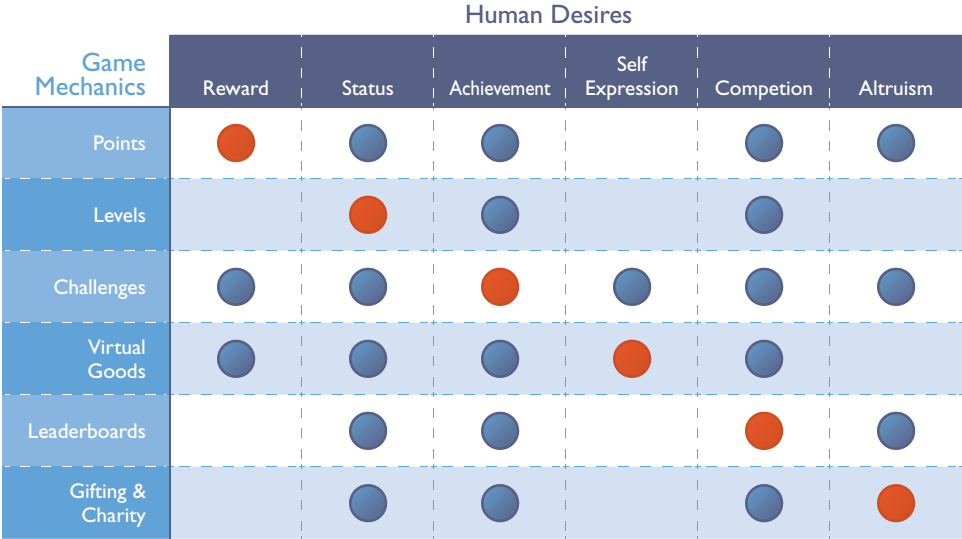
\includegraphics[width=\textwidth]{img/bunchball.png}
  \caption{Interaction between Human desires and Game mechanics}
  \label{fig:bunchball}
\end{figure}\todo{Source + explain why some balls are blue and why others are red}

\todo{New material for Martin}As can be seen, the human desires can be fulfilled via various game mechanics.
FoldIt utilizes a leaderboard, which allows the users to compete against each other either as groups or soloists. Allowing both groups and soloists to competes makes the game both appealing to individualists and team players. If only groups could compete, it might impact the amount of individualists that would participate. We see, that appealing to a wider range of character types increase the number of people that use the game. This is something, that should be taken into account when developing our game.\newline

In the online application FreeRice, developed for the World Food Program, the user's desire for altruism/selflessness is fulfilled via donations of rice grains for completed tasks, while general academic skills are honed, such as vocabulary and basic mathematical proficiency. Again, it is possible to join groups, and it game also utilize a leaderboard, thereby introducing the competition desire.\cite{freerice}\newline

As has been described, the game mechanics in Figure \ref{fig:bunchball} will give people an extrinsic motivation (rewards, leaderboards etc.) to keep playing, although the activity might not carry any intrinsic motivation for the user. This is useful in education, because people tend to easily give up, or simply never really start, when acquiring knowledge and skills that, while useful, may not be their primary field of interest. Keeping people entertained while learning can ensure that they spend more time on the subject and may also pique their interest in an area they might not have explored by themselves. \todo{New material for Martin}We also see that challenges is the only game mechanic to engage all the human desires, which is why challenges should be introduce earlier than for example levels and leaderboards. However, all game mechanics should be considered and the complexity of implementing one game mechanic over another also has an impact on the time it will be implemented. For example, a game mechanic that can easily be implemented, but does not fulfill very many human desires may be implemented before a more fulfilling game mechanic.
